\documentclass[12pt]{report}
\usepackage[spanish,es-nosectiondot,es-lcroman]{babel}
\usepackage{siunitx}
\usepackage[utf8]{inputenc}
\usepackage{amsmath}
\usepackage{float}
\usepackage{listings}
\usepackage{xcolor}
\usepackage{amssymb}


\usepackage{graphicx}
\usepackage{hyperref}
\usepackage{geometry}
%Configuracion para el . en decimales
\sisetup{output-decimal-marker = {.}}
% Configuración para el código
\lstset{
	language=Python,
	basicstyle=\ttfamily\footnotesize,
	numbers=left,
	numberstyle=\tiny\color{gray},
	stepnumber=1,
	numbersep=10pt,
	backgroundcolor=\color{white},
	showspaces=false,
	showstringspaces=false,
	showtabs=false,
	frame=single,
	rulecolor=\color{black},
	tabsize=4,
	captionpos=b,
	breaklines=true,
	breakatwhitespace=false,
	linewidth=\linewidth,
	keepspaces=true,
	columns=flexible,
	keywordstyle=\bfseries\color{blue},
	commentstyle=\itshape\color{lightgray},
	stringstyle=\color{red},
	escapeinside={\%*}{*)},
}

% Configuración de los márgenes
\geometry{
	left=2cm,   % Margen izquierdo
	right=2cm,  % Margen derecho
	top=2cm,    % Margen superior
	bottom=2cm  % Margen inferior
}

% Title Page
\title{Machine Learning para mineria de datos\\
	Homework 1}
\author{Salazar Martinez Miguel Angel}

\begin{document}
	\renewcommand{\arraystretch}{1.3}
	
	\maketitle
	
\begin{figure}[H]
	\centering
	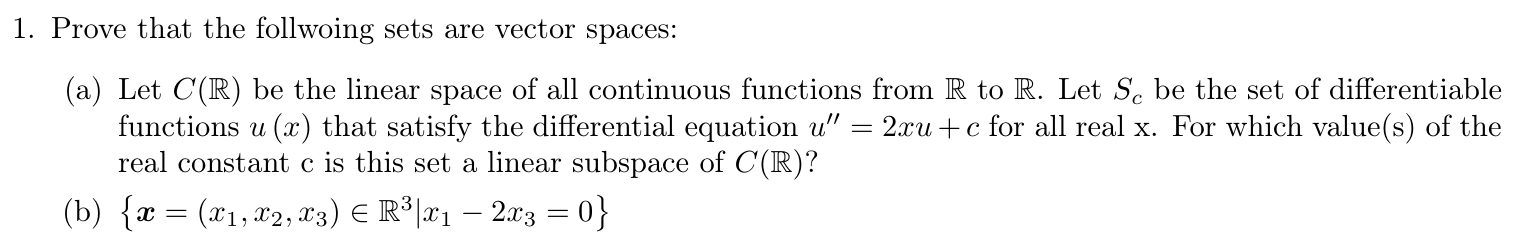
\includegraphics[width=1\textwidth]{inciso1}
\end{figure}
Respuesta:


(a) 

Consideremos el conjunto \( S_c \) de funciones diferenciables \(u(x) \) que satisfacen la ecuación diferencial \( u'' = 2xu + c\). Para que \( S_c \) sea un subespacio de \( C(\mathbb{R}) \), debemos verificar las propiedades de subespacio:

- Cerradura bajo la suma: Sean \( u_1, u_2 \in S_c \), entonces \( u_1'' = 2xu_1 + c \) y \( u_2'' = 2xu_2 + c \). Sumando ambas ecuaciones:
\[
(u_1 + u_2)'' = 2x(u_1 + u_2) + 2c.
\]
Para que \( S_c \) sea cerrado bajo la suma, debemos tener \( 2c = c \), lo que implica \( c = 0 \).

- Cerradura bajo la multiplicación por escalares: Sea \( u \in S_c \) y \( k \in \mathbb{R} \). Entonces, \( u'' = 2xu + c \). Al multiplicar por \( k \):
\[
(ku)'' = 2x(ku) + kc.
\]
Para que \( kc = c \), debe ser \( c = 0 \).

- Contiene el vector cero: La función cero \( u(x) = 0 \) satisface \( u'' = 2x \cdot 0 + c \) solo si \( c = 0 \).

Por lo tanto, \( S_c \) es un subespacio solo si \( c = 0 \).

(b) 

Sea \( S = \{ x = (x_1, x_2, x_3) \in \mathbb{R}^3 \mid x_1 - 2x_3 = 0 \} \). Verifiquemos si \( S \) es un subespacio:

- Cerradura bajo la suma: Sean \( x, y \in S \), es decir, \( x_1 - 2x_3 = 0 \) y \( y_1 - 2y_3 = 0 \). Entonces:
\[
(x_1 + y_1) - 2(x_3 + y_3) = (x_1 - 2x_3) + (y_1 - 2y_3) = 0.
\]
Por lo tanto, \( x + y \in S \).

- Cerradura bajo la multiplicación por escalares: Sea \( k \in \mathbb{R} \) y \( x \in S \), es decir, \( x_1 - 2x_3 = 0 \). Entonces:
\[
(kx_1) - 2(kx_3) = k(x_1 - 2x_3) = 0.
\]
Por lo tanto, \( kx \in S \).

- Contiene el vector cero: El vector cero \( (0, 0, 0) \) satisface \( x_1 - 2x_3 = 0 \).

Por lo tanto, \( S \) es un subespacio de \( \mathbb{R}^3 \).

\begin{figure}[H]
	\centering
	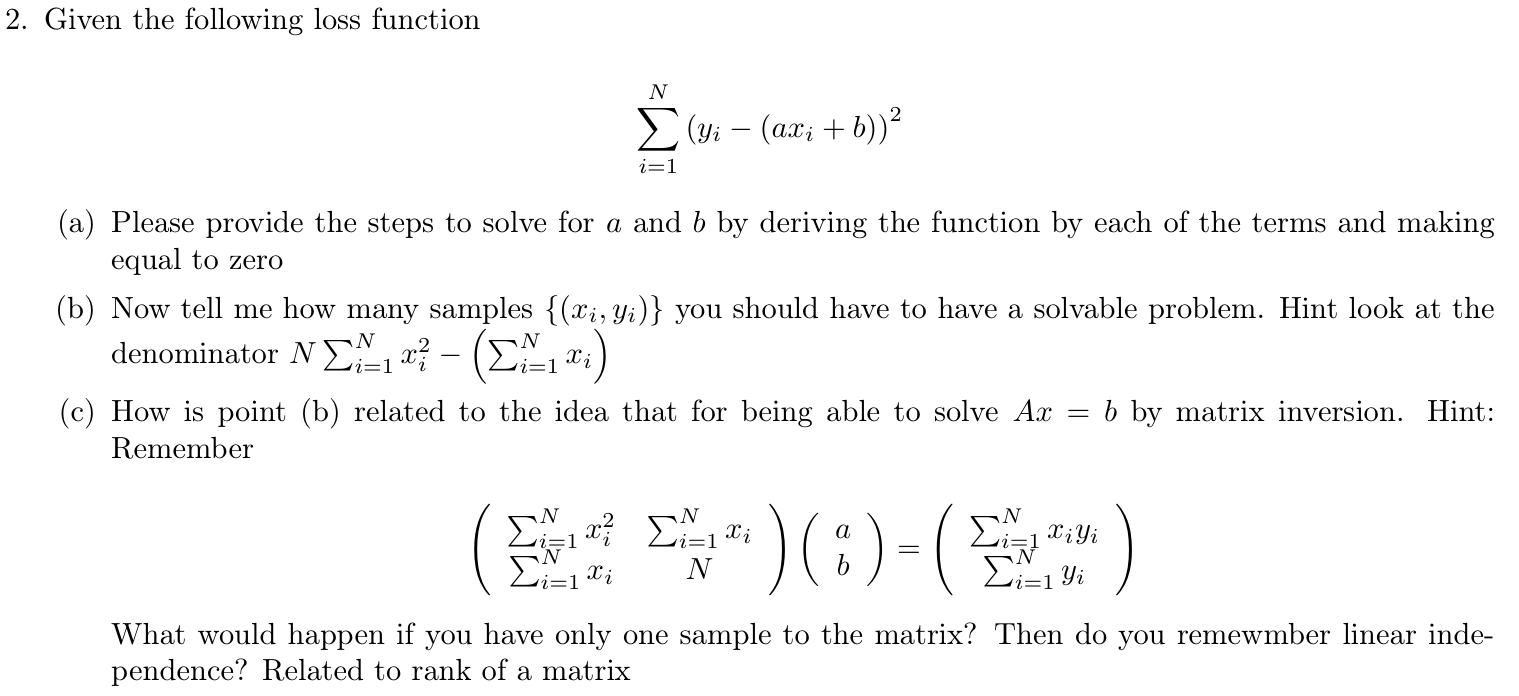
\includegraphics[width=1\textwidth]{inciso2}
\end{figure}
Respuesta:


(a) 

La función de pérdida es:
\[
L(a, b) = \sum_{i=1}^{N} \left( y_i - (ax_i + b) \right)^2.
\]
Para encontrar los valores óptimos de \( a \) y \( b \), derivamos respecto a \( a \) y \( b \) y igualamos a cero.

1. Derivada respecto a \( a \):
\[
\frac{\partial L}{\partial a} = \sum_{i=1}^{N} -2x_i \left( y_i - (ax_i + b) \right).
\]
Igualando a cero:
\[
\sum_{i=1}^{N} x_i \left( y_i - (ax_i + b) \right) = 0.
\]

2. Derivada respecto a \( b \):
\[
\frac{\partial L}{\partial b} = \sum_{i=1}^{N} -2 \left( y_i - (ax_i + b) \right).
\]
Igualando a cero:
\[
\sum_{i=1}^{N} \left( y_i - (ax_i + b) \right) = 0.
\]

(b) 

La condición para que el problema sea resolvible es que el determinante de la matriz asociada no sea cero:
\[
N \sum_{i=1}^{N} x_i^2 - \left( \sum_{i=1}^{N} x_i \right)^2 \neq 0.
\]
Esto requiere al menos dos valores distintos de \( x_i \). Si todos los \( x_i \) son iguales, la matriz sería singular.

(c) 

El problema puede escribirse en la forma \( Ax = b \), donde:
\[
A = \begin{pmatrix}
	\sum_{i=1}^{N} x_i^2 & \sum_{i=1}^{N} x_i \\
	\sum_{i=1}^{N} x_i & N
\end{pmatrix},
\quad
x = \begin{pmatrix}
	a \\
	b
\end{pmatrix},
\quad
b = \begin{pmatrix}
	\sum_{i=1}^{N} x_i y_i \\
	\sum_{i=1}^{N} y_i
\end{pmatrix}.
\]
Si solo hay una muestra, \( \det(A) = 0 \) y \( A \) no es invertible, lo que está relacionado con la independencia lineal y el rango de la matriz.

\begin{figure}[H]
	\centering
	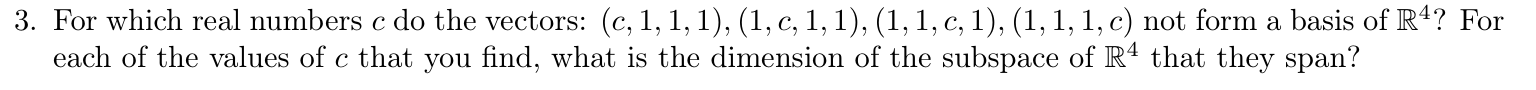
\includegraphics[width=0.9\textwidth]{inciso3}
\end{figure}
	Respuesta:
	
	
	Los vectores son:
	\[
	v_1 = (c, 1, 1, 1), \quad v_2 = (1, c, 1, 1), \quad v_3 = (1, 1, c, 1), \quad v_4 = (1, 1, 1, c).
	\]
	Forman una base si \( \det(A) \neq 0 \), donde:
	\[
	A = \begin{pmatrix}
		c & 1 & 1 & 1 \\
		1 & c & 1 & 1 \\
		1 & 1 & c & 1 \\
		1 & 1 & 1 & c
	\end{pmatrix}.
	\]
	Calcula \( \det(A) \) y encuentra para qué valores de \( c \) es cero. Esos valores indican cuando los vectores no forman una base. La dimensión del subespacio generado dependerá del rango de \( A \).
	
	
	
\begin{figure}[H]
	\centering
	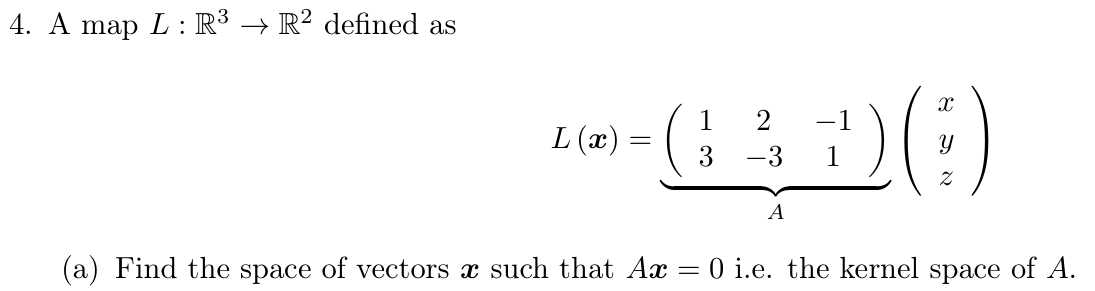
\includegraphics[width=0.9\textwidth]{inciso4}
\end{figure}
Respuesta:


La transformación lineal \( L : \mathbb{R}^3 \to \mathbb{R}^2 \) está definida por:
\[
L(x) = \begin{pmatrix}
	1 & 2 & -1 \\
	3 & -3 & 1
\end{pmatrix} \begin{pmatrix}
	x \\
	y \\
	z
\end{pmatrix}.
\]
Para encontrar \( \ker(L) \), resuelve \( Ax = 0 \):
\[
\begin{pmatrix}
	1 & 2 & -1 \\
	3 & -3 & 1
\end{pmatrix} \begin{pmatrix}
	x \\
	y \\
	z
\end{pmatrix} = \begin{pmatrix}
	0 \\
	0
\end{pmatrix}.
\]
El sistema no tiene solución, ya que al intentar representarlo como un sistema de ecuaciones se obtiene lo siguiente:

\[
x + 2y - z = 0
\]
\[
3x - 3y + x = 0
\]

Lo cual resulta en un sistema que no es posible resolver, ya que se trata de un sistema incompleto.



\begin{figure}[H]
	\centering
	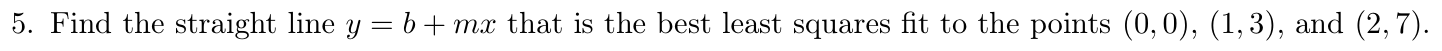
\includegraphics[width=1\textwidth]{inciso5}
\end{figure}
	Respuesta:
	
	NOTA: La recta calculada no pasa por el origen, supongo que fue un error de dedo.
	
	Dado los puntos \( (0, 0), (1, 3), (2, 7) \), ajusta la línea \( y = mx + b \),seguimos los siguientes pasos:
	
	1. Identificar los puntos: Los puntos dados son \((0,0)\), \((1,3)\) y \((2,7)\).
	
	2. Extraer las coordenadas:
	\[
	\text{Punto 1: } (x_1, y_1) = (0, 0)
	\]
	\[
	\text{Punto 2: } (x_2, y_2) = (1, 3)
	\]
	\[
	\text{Punto 3: } (x_3, y_3) = (2, 7)
	\]
	
	3. Calcular la pendiente (\(m\)):
	Para calcular la pendiente, utilizamos la fórmula:
	\[
	m = \frac{y_2 - y_1}{x_2 - x_1}
	\]
	Usando los puntos \((1,3)\) y \((2,7)\):
	\[
	m = \frac{7 - 3}{2 - 1} = \frac{4}{1} = 4
	\]
	
	4. Calcular la ordenada al origen (\(b\)):
	Usamos la ecuación de la recta \(y = mx + b\) con la pendiente \(m = 4\) y uno de los puntos. Usamos el punto \((1,3)\):
	\[
	3 = 4(1) + b
	\]
	\[
	3 = 4 + b \quad \Rightarrow \quad b = 3 - 4 = -1
	\]
	
	5. La ecuación de la recta:
	La ecuación de la recta es:
	\[
	y = 4x - 1
	\]
	
	
	
\end{document}

